  \documentclass[12pt,oneside]{article}
  \title{Fundamentals of rough volatility models.}
  \date{March 2021}
  \author{Rachel Dance, Tim Howes, Silvia Cecilia Hernández Vargas, Finlay Young}
  \usepackage{graphicx}
%   \usepackage{cleveref}
  \usepackage[citation-order]{amsrefs}
  \usepackage[rsfm,fancyhdr,hyperref,colour]{edmaths_mod}
  \flushbottom

  \begin{document}
  \pagenumbering{roman}
  \maketitle

  \begin{abstract}The aim of this report is to bring together and summarise the key works leading to the inception of rough volatility models, and note recent advances to make implementation feasible. This work focuses on the theoretical background driving the `rough' volatility models, and how they arose. Key results from empirical market analysis that have been used to motivate the consideration of volatility as a `rough' process are discussed \cite{Gatheral2014}. We present how rough volatility can be used for pricing options, and give an overview of two well documented examples of this type of model that provide a better fit to market volatility data. Given that simulation of rough volatility models tends to be slow, this work provides a brief account of the computational advancements which allow these models to be tractable and computationally efficient.
  \end{abstract}

  \tableofcontents
 \newpage
 \pagenumbering{arabic}

\section{Introduction}
The financial industry has always sought better models to improve market replication. In particular, to obtain better accuracy in pricing derivatives contracts, the underlying asset behaviour must be correctly modelled. One of the most important parameters in achieving this goal is the volatility parameter. Empirical evidence has shown that the volatility is not a constant parameter, which the Black-Scholes model considers as an assumption, and can be thought of as a stochastic process.
\\

Models to estimate the volatility can be divided into historical models and implied volatility models, where the latter derives the volatility of the underlying asset from the option price observed in the market. On the other hand, stochastic models (which fall into the historical models category) have made great improvements in capturing characteristics observed in market volatility, as they can model continuous-time dynamics for the volatility process. However, they tend to differ when comparing to the observed dynamics in the market. For example, stochastic volatility models such as the Hull and White, Heston and SABR models generate the implied volatility surfaces with different shapes as those observed in the market. 
\\

In order to produce a better replication of the volatility process seen in the market, Rough Volatility models were introduced. Rough volatility models are driven by a fractional Brownian motion (fBm), which incorporates the non-Markovian noise into the volatility process that is observed in market data. The inclusion of fBm with Hurst parameter $H\in(0,1/2)$ also introduces into the model the empirically observed `rough' smoothness properties of the volatility process. The term (`rough'), originally coined by Gatheral et al.\cite{Gatheral2014} in their seminal work on the matter, has become synonymous with modelling volatility as a stochastic process in its own right, and how this is incorporated into models and implemented, continues to be an active area of research. In particular, the non-Markovian property of fBm essentially restricts pricing methods under Rough Volatility models to Monte Carlo simulation, which can generally be quite slow. Advancements in this area of numerical approximation such as the Hybrid Scheme \cite{Bennedsen2017} and an extension of Donsker's theorem to fBm \cite{Horvath2017} have provided some solutions to this computational burden, with work still progressing in this particular area of research.
\\

This review is structured as follows. In Section~\ref{sec:black_scholes_foundations} we summarise the theoretical foundations of volatility models and give a brief overview of fBm. In Section~\ref{sec:rough_volatility}, we discuss the evidence of rough volatility in the market, pricing with rough volatility models and provide a detailed discussion of both the Rough Bergomi and Rough Heston models. In Section~\ref{sec:comp_advancement}, we give an outline of relevant advancements in numerical methods that allow rough volatility models to be feasible. We conclude with Section~\ref{sec:summary&futurework} in which we provide some final remarks.

\section{Theoretical foundations}
\label{sec:black_scholes_foundations}

The Black and Scholes (BS) model was first introduced in the 1970's as an improvement to the very early work by Bachelier \cite{Bachelier1900}, and is arguably the most well known option pricing model \cite{BlackScholes1973}. It is a fundamental building block of almost all current pricing models, but it is rarely used directly due to its well known and documented shortcomings. Therefore we give a short overview as a precursor to the remaining discussion of this report.
\\

The price of an option ($S_t$) at a time $t$ is not generally expected to remain at its current value for long periods. Broadly speaking, the value of any asset will increase (or decrease) on average by some rate $\mu\in\mathbb{R}$. The BS model also contains a volatility term $\sigma$, representing the variability of the price of an asset in the short term. The model takes the form of Equation \ref{eqn:black_and_scholes}.

\begin{equation}
\label{eqn:black_and_scholes} 
dS_t=\mu S_t dt + \sigma S_t dW
\end{equation}

In this model, W is a Wiener process with normally distributed increments, and it dictates that the log price $S_t$ is a stochastic process that is continuous in time. As such, $S_t$ also follows a Brownian Motion, where the dt term is the drift and $\sigma$ the diffusion of the process. 
\\

The key shortcomings of the model are firstly that $\mu$ and $\sigma$ are represented either as constants, or as deterministic functions of time \cite{BlackScholes1973, Gatheral2014}. In the context of this report, this is very important as empirical evidence shows that the volatility is not constant. As an example, a quadratic relationship between implied volatility and strike price of an option for a given maturity, which became known as the `volatility smile'. This function can vary depending on the type of the market, e.g. for equity or foreign markets, and is a well known and documented topic in the literature \cite{Hull2015}.
\\

Volatility estimation can be broadly put into two related but distinct classes, historical and implied volatility. Implied volatility model is also known as forward looking model, where the implied volatility can be defined as the parameter needed for a theoretical model, such as the BS model, to have the same option price as the one observed in the market.
\\

A historical estimation model, also known as backward looking model, uses the historical data as the main input to estimate the volatility of a given asset. One example of a historical model is the standard deviation (single point estimate). However, this method does not capture the whole dynamic of the volatility process like the Stochastic models do, where they allow volatility to be a stochastic process. Stochastic models fall into the parametric category where we assume a distribution for our data. Nevertheless, the estimation of model parameters can be challenging and computational tractability is a key factor. However, with the advent of accessible neural network technologies and recent developments in numerical methods for solving these types of problems \cite{Horvath2019}, it is anticipated that these models will become ever more popular as they have evolved to have a better accuracy of the market data.
\\

In the following sections, we introduce a popular stochastic model for volatility, and a subsequent improvement of this model. This extends the BS model significantly by considering volatility as a stochastic process in its own right, and further, observing the increments of Brownian motions as correlated, as was not done thus far. Armed with this, we are adequately prepared to describe how the rough volatility model is formed.


\subsection{The Heston Model}
The Heston model is a popular parametric stochastic volatility model which allows for European option pricing, and was developed as an improvement on the Black-Scholes (BS) model in the 1990s \cite{Douglas1993}. The main difference between the Heston model and BS model is the additional randomness introduced by the consideration of volatility as a stochastic process and the non standard normal distribution of the stock returns. With this modification, we can now take into account the fat tails observed in the stock return distribution and the volatility smile explained in the previous section. In the BS model, volatility is a constant value which provides a simplistic model, but it is not a realistic representation of asset volatility in the market. In the Heston model the underlying asset volatility is modelled by the Cox-Ingersoll-Ross model (CIR, commonly used as an interest rate model). The Heston model is outlined below in Equation \ref{eqn:classic_heston}.

\begin{equation}
\label{eqn:classic_heston}
dS_t= S_t(\mu dt + \sqrt{v_t} dW_t^{s})
\end{equation}
where the variance is expressed as: 
\begin{equation}
\label{eqn:classic_heston_var}
dv_t = \kappa (\theta - v_t)dt + \xi\sqrt{v_t}dW_t^{v}
\end{equation}

As we can see in the above, the volatility from the BS model, $\sigma$ is replaced with the square root of variance, which is now a process. The parameters for the dynamic of the variance can be interpreted as: $\xi$, the `volatility of volatility' which allows for control of the curvature of the volatility smile, $\kappa$, the rate at which $v_t$ returns to 0 (the mean reversion); and $\theta$ which is the long-running price variance. 
\\

The Heston model has two Brownian motion components, one corresponding to the asset price ($W^s$), and one corresponding to the asset variance ($W^v$). From It\^o isometry we have $\langle  dW_t^{s} dW_t^{v}\rangle$ = $\rho dt$, where $\rho$ is the correlation coefficient for these two Brownian motions.
\\

However, from a time series modelling point of view, stochastic volatility models, such as the Heston model have been criticised for not taking into account the long memory of the observed volatility of returns. Therefore, to include this characteristic, the fBM model was developed. 

\subsection{Fractional Brownian Motion}
\label{sec:fractionalBm}
In addition to describe the improvement made for modelling the volatility, as mentioned before, it is important to introduce the concept of fractional Brownian Motion (fBM). fBm is a fundamental component of rough volatility models described in Section \ref{sec:rough_volatility}. The key  advantage in fBm, is that the increments of the process are not necessarily independent, thus the process cannot be considered Markovian. The inclusion of fBm originates from the analysis of empirical time series data which suggests that the volatility process is non-Markovian, and possesses certain smoothness properties, as is further detailed in \cite{Gatheral2014}. As such, fBM can be written as a stochastic process $(W^H_t)_{t\ge0}$ where \textit{H} is called the Hurst parameter with $\textit{H} \in (0,1)$. Similar to the classical Brownian motion, it has the following properties: 
\begin{enumerate} 
\item The process is Gaussian and H\"{o}lder-continuous in time. 
\item $(\textit{$W^H_0$})=0$  
\item $\mathbb{E}$[\textit{$W^H_t$}]$=0$,
$\forall t \ge 0$ 
\end{enumerate}

 By looking at the properties of fBM, we can see how it would be preferred over classical Brownian motion, and how it satisfies the non-Markovian time series property. It differs from the classical Brownian motion as it has covariance function given by Equation \ref{eqn:fBMcov}.
\begin{equation}
\label{eqn:fBMcov}
\mathbb{E}[W^H_{t_1}W^H_{t_2}]=1/2(|t_1|^{2H}+|t_2|^{2H}-|t_1-t_2|^{2H})
\end{equation}

If $H=1/2$ the covariance becomes 0, meaning that increments are not correlated, giving us the classical Brownian motion. If $H<1/2$ then the covariance is negative, meaning the increments of the process are negatively correlated. Finally, if $H>1/2$ then the covariance is positive, meaning the increments of the process are positively correlated. Therefore, by setting $H\in(0,1)\setminus\{\frac{1}{2}\}$, we allow for dependence between the increments of fBM. Hence, by modelling the volatility process to be driven by fBm with $H\in(0,1)\setminus{1/2}$ the volatility process becomes non-Markovian.
\\

Now we are ready to introduce the concept of rough volatility models which gives volatility a short memory property, thus contradicting the largely accepted fact that the volatility process is long memory.

\section{Rough volatility}
\label{sec:rough_volatility}

The main motivation for developing what is now known as `rough volatility' was to produce a model which would bridge the gap between the volatility surface generated by conventional stochastic volatility models, to the surfaces generated by observed (historical) volatility, thus having a better fit to the observed market.
\\

In Section \ref{sec:rough_vol_evidence}, we discuss the evidence for rough volatility in the market, in Section \ref{sec:Pricing} we discuss pricing under rough volatility models and in Sections \ref{sec:rough_Bergomi} and \ref{subsec:rough_heston}, we discuss the construction of the Rough Bergomi model and the Rough Heston Model respectively. 

\subsection{Evidence of Rough volatility in the Market}
\label{sec:rough_vol_evidence}
 
Evidence to support the accuracy of the rough volatility  has been well explored by Gatheral et al. \cite{Gatheral2014}, where the smoothness and increments of the log-volatility process for selected assets were investigated. It was shown that empirically, the increments of the log-volatility process exhibit a scaling property in expectation with a constant smoothness parameter $H$, given by Equation \ref{eqn:scaling_prop}, 

\begin{equation}
\label{eqn:scaling_prop}
\mathbb{E}[|log(\sigma_\Delta)-log(\sigma_0)|^q]=K_q\nu^q\Delta^{qH}
\end{equation}

where $\Delta$ is the increment size, $q>0$ and $\nu>0$. Moreover, fBm enjoys a scaling property almost identical to Equation \ref{eqn:scaling_prop}. The distribution of the increments was also shown to be  approximately Gaussian, leading  to a proposed model for the asset price and volatility process using fractional Brownian motion given by Equations \ref{eqn:rough_asset}, \ref{eqn:roughvol}, and \ref{eqn:OU_rough}.

\begin{equation}
\label{eqn:rough_asset}
 \frac{dS_{t}}{S_{t}} = \mu_{t} dt + \sigma_{t} dZ_{t},
\end{equation}
\begin{equation}
\label{eqn:roughvol}
    \sigma_{t} = exp(X_{t}),
\end{equation}

\begin{equation}
\label{eqn:OU_rough}
X_{t}=\vega\int_{-\infty}^{t} e^{-(t-s)\alpha}dW_{t}^{H}+m,
\end{equation}

where $\mu_{t}$ is the drift term, $Z_{t}$ is a standard Brownian Motion, $X_{t}$ is a fractional Ornstein–Uhlenbeck process with $\alpha>0$, $m\in\mathbb{R}$ and $0<H<1/2$ is the measured smoothness of the volatility. We should also mention that $Z$ and $W^{H}$ are correlated in general. This model was coined the Rough Fractional Stochastic Volatility (RFSV) model. It is important to note that for the purpose of this section, we are not interested in this model specifically, but rather the smoothness and fractal properties it possesses.
\\

Comparison of the smoothness of simulated data from this model to that of empirical data, provides ample evidence that volatility is indeed rough. A key part of this analysis was comparing the actual volatility of the S\&P over a 3500 day period with the volatility process generated by the model over the same time-frame. The results of which are shown in Figure \ref{fig:gatheral_2014_volplots}.
\\

\begin{figure}[htpb]
    \centering
    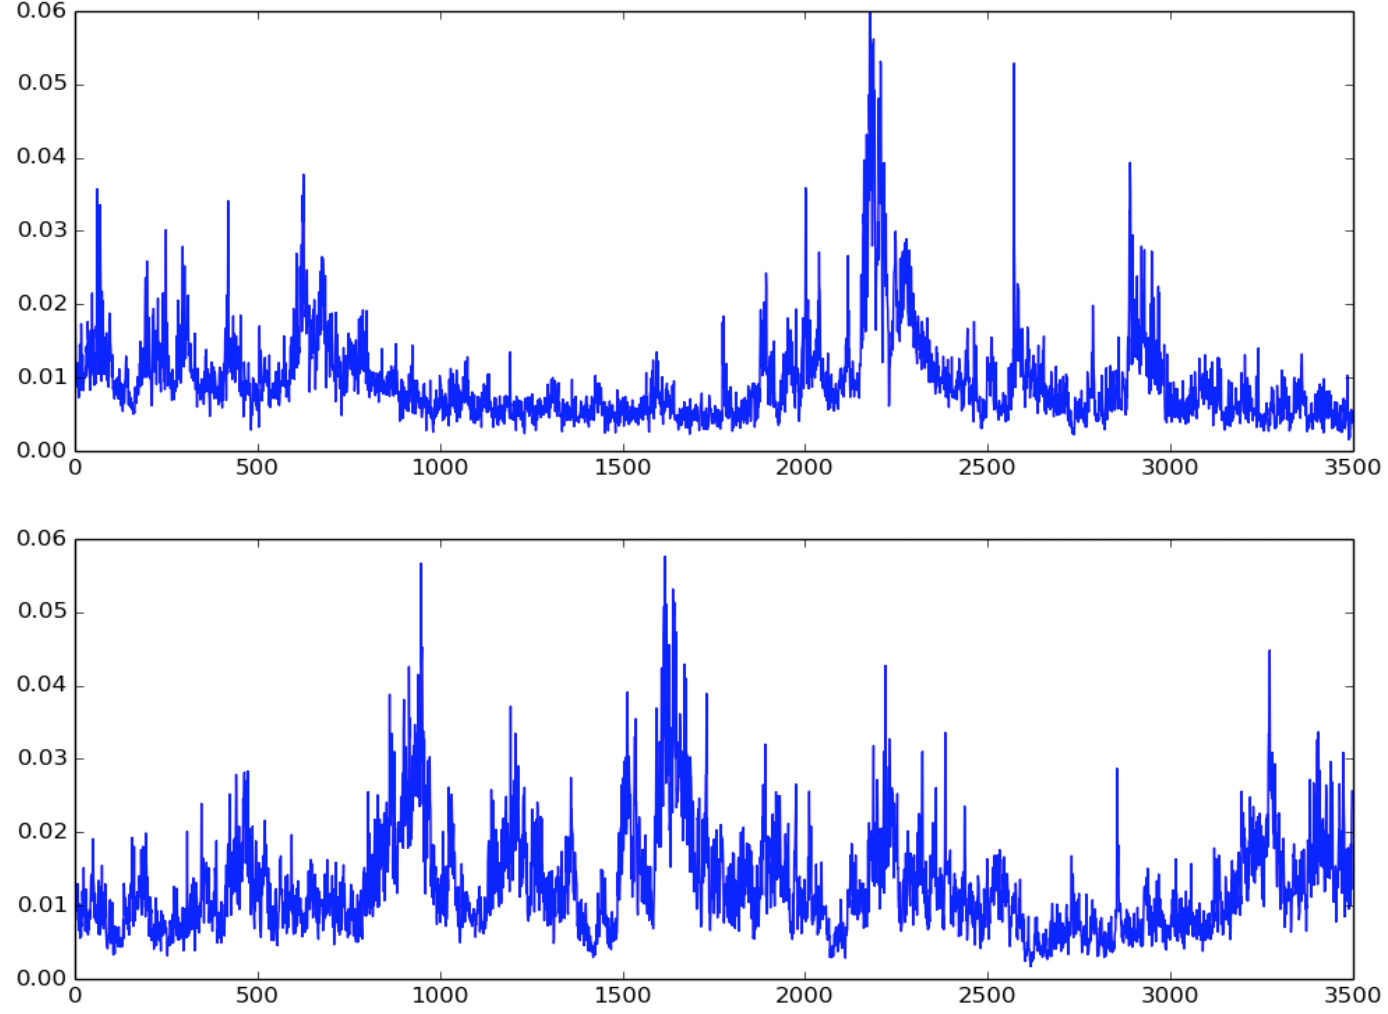
\includegraphics[width=0.85\textwidth ]{figs/Gatheral2014_fig36_p22}
    \caption{Extracted directly from Gatheral et al., 2014, \cite[Figure~3.6]{Gatheral2014}. Sample path of the model generated volatility (bottom) compared with the S\&P volatility (top). The x-axis represents the time in days, and the y-axis represents volatility.}
    \label{fig:gatheral_2014_volplots}
\end{figure}

As is highlighted in \cite{Gatheral2014}, we observe a striking similarity between both plots of Figure \ref{fig:gatheral_2014_volplots}, with both exhibiting periods of high volatility, followed or preceded by periods of low volatility. Recall that choosing $H<1/2$ means that the increments of the fractional Brownian motion are negatively correlated. In this analysis, $H$ was chosen to be less than 1/2 which would capture this certain trend in the model, as was discussed in Section \ref{sec:fractionalBm}. The smoothness of the volatility process could be captured through this model by tuning $H$.
\\

It is important to mention that RFSV model is not long memory. However, when applying standard statistical estimators to data simulated by the RFSV model, long memory was incorrectly found to be present, with parameters estimated similar to those found in other studies. This led Gatheral et al. to conclude that this is why volatility having a long memory property is often accepted as a stylised fact. 
\\

A more recent paper \cite{Fukasawa2020} also showed that volatility has to be rough through an arbitrage argument, involving the power law associated with implied volatility which is empirically observed in option markets \cite{Carr2001}. The power law of implied volatility, also known as the `volatility smirk', aims to approximate the implied volatility curve of some options, which have a higher implied volatility for low strikes and a lower implied volatility for higher strikes. This shape is shown to be a negative skew, where the curve is steep for low strikes and flattens out for higher strikes (hence the name `volatility smirk'). Fukusawa \cite{Fukasawa2020} shows that there is an arbitrage opportunity if volatility isn't rough given an option market obeying the power law given in Equation \ref{eqn:powerlaw},

\begin{equation}
\label{eqn:powerlaw}
\frac{\sigma_{BS}(K,T) - \sigma_{BS}(K',T)}{K-K'}\propto T^{H-1/2}
\end{equation}

where $K \approx 0$, $K' \approx 0$, with $H \approx 0$ when $T \approx 0$. Here, $\sigma_{BS}(K,T)$ is the Black-Scholes implied volatility with log-moneyness $K$ and time to maturity T. This arbitrage opportunity is under the assumption that the asset price is a positive continuous It\^o semi-martingale.
\\

Further studies have explored the origin of rough volatility, and it is considered to be a consequence of the no arbitrage principle and market impact \cite{Jusselin2018}. In this context, market impact is defined to be the fact that on average for a given asset, a buy order increases it's price and a sell order causes a decrease in it's price. Given the overwhelming evidence discovered through such studies, it has been thoroughly accepted as a stylized fact that volatility is indeed rough.

\subsection{Pricing with Rough Volatility Models}
\label{sec:Pricing}
In this section, we describe how Rough Fractional Stochastic Volatility models can be used to price contingent claims and thus for option pricing. We first discuss the method of pricing under the physical measure $\mathbb{P}$, and then under the risk-neutral measure $\mathbb{Q}$. 

\subsubsection{Pricing under the Physical Measure, \mathbb{P}}

As stated in the previous section, the distribution of increments of the logarithm of realized variance were found to be close to Gaussian, which motivates the use of a model where $\sigma_{t}$ is treated as a log-normal random variable. The time series of the realised variance was proposed to be modelled by:

\begin{equation}
\label{eq:realizedvariance}
    log\sigma_{t+\Delta} - log\sigma_{t} = \nu (W_{T+\Delta}^{H} - W_{t}^{H})
\end{equation}

where $W^{H}$ is fBM.
Now, consider the Mandelbrot-Van Ness representation of fBM $W_{H}$ \cite{Mandelbrot1968}:

\begin{equation}
\label{eq:mandelbort}
    W_{t}^{H} = C_{H} \left[ \int_{-\infty}^{t} \frac{dW_{s}^{P}}{(t-s)^{\gamma}} - \int_{-\infty}^{0} \frac{dW_{s}^{P}}{(-s)^{\gamma}}\right]
\end{equation}

In particular, if we choose $\gamma = 0.5-H$ and $C_{H} = \sqrt{\frac{2H\Gamma(3/2- H)}{\,\Gamma\,(H+0.5) \Gamma(2-2H)}}$, then we can ensure the property of the covariance of fBM stated in [\ref{eqn:fBMcov}].
\\

Let us substitute [\ref{eq:mandelbort}] into [\ref{eq:realizedvariance}], then the evolution of the instantaneous variance $\nu_{u}$ under the physical measure P would be:
\begin{equation}
    log\upsilon_{u} - log\upsilon_{t} := 2  \nu\, [M_{t}(u) + Z_{t}(u)]
\end{equation}

Here, $M_{t}(u)$ is independent of $\mathcal{F}_{t}$ with mean zero and variance $(u-t)^{2H} /(2H)$, and $Z_{t}(u)$ is $\mathcal{F}_{t}$-measurable.
\\

Let us introduce  $\tilde{W_{t}^{P}(u)}$ which has the same properties as $M_{t}(u)$ but with different variance:

\begin{equation}
    \tilde{W_{t}^{P}(u)}:= \sqrt{2H} \int_{t}^{u} \frac{dW_{s}^{P}}{(u-s)^\gamma}
\end{equation}

With $\eta := 2 \nu C_{H}/ \sqrt{2H}$ we have $2\eta C_{h} M_{t}(u) = \eta \tilde{W_{t}^{P}(u)}$, so we can write the instantaneous variance as:
\begin{equation}
\label{eq:volunderP}
\begin{split}
    \upsilon_{u} & = \upsilon_{t} \exp{(\eta\; \tilde{W_{t}^{P}(u)} + 2\eta\,C_{H}\,Z_{t}(u))} \\
    & = \mathbb{E}^{P} [\upsilon_{u}| \mathcal{F}_{t}] \,\varepsilon\, (\eta \tilde{W_{t}^{P}(u)})
\end{split}
\end{equation}
 
 where $\varepsilon$ is defined as the "Wick" exponential. This model is defined using two standard Brownian motions $Z^{P}$ and $W^{P}$ with a constant correlation $\rho$. We can see that the conditional distribution of $\upsilon_{u}$ depends on $\mathcal{F}_{t}$ but only through the variance forecasts $E^{P} [\upsilon_{u}| \mathcal{F}_{t}]$. Therefore, in order to price options, we do not need to know the $\mathcal{F}_{t}$.
\\

It is important to recall that the dynamic of the price would be:
\begin{equation}
     \frac{dS_{u}}{S_{u}} = \mu_{t}\, du + \sqrt{\upsilon_{u}}\,dZ_{u}^{P},
\end{equation}

\subsubsection{Pricing under the Risk-Neutral Measure, \mathbb{Q}}

To price options we need an equivalent martingale measure such that the discounted prices process $S_{t}$ is a martingale under this new measure, i.e changing from measure P to measure Q.

The following changes of measure are done:

\begin{equation}
    dZ_{u}^{Q} = dZ_{u}^{P} + \frac{\mu_{u}}{\sqrt{\upsilon_{u}}}du
\end{equation}

where $ t \leq u \leq T$, and:

\begin{equation}
    dW_{u}^{Q} = dW_{u}^{P} + \left[\frac{\rho \mu_{u}} {\sqrt{\nu_{u}} + \rho \gamma_{u}}\right] du
\end{equation}

In fact, let consider a general change of measure of the style:

$$dW_{s}^{P} = dW_{s}^{Q} + \lambda_{s} ds$$

with this visualisation, we can interpret $\lambda$ as the price of volatility risk. In this sense, we can rewrite [\ref{eq:volunderP}] as:

\begin{equation}
\label{eq:volunderQ}
    \upsilon_{u} & = E^{P} [\upsilon_{u}| \mathcal{F}_{t}]\, \varepsilon\, ( \eta\, \tilde{W_{t}^{Q}}(u))\; exp \left[\eta \sqrt{2H} \int_{t}^{u} \frac{\lambda_{s}}{(u-s)^{\gamma}} ds\right]
\end{equation}

\subsection{The Rough Bergomi Model}
\label{sec:rough_Bergomi}
In this subsection, the Bergomi model is transformed into a Rough Bergomi Model, which has showed to fit the SPX volatility better than conventional Markovian stochastic models \cite{Bayer2016}.
\\

A relevant characteristic which distinguish among different volatility models is the term structure of the ATM volatility skew, defined as:

\begin{equation}
    \psi(\tau) = \Big| \frac{\partial}{\partial k} \sigma_{BS}(k,\tau) \Big|_{k = 0}
\end{equation}

where $\tau = T - t$ is the time to maturity, and $k$ is the log-moneyness equal to $log(\frac{K}{S_{t}})$. Stochastic models present the ATM volatility skew to be constant for short dates and inversely proportional to $\tau$ for long dates. We can see in Figure \ref{fig:Bayer2016_vol_skew} how the skew volatility is proportional to $\tau^{-\alpha}$, for $0\leq \alpha \leq 1/2$. 
\\

\begin{figure}[htpb]
    \centering
    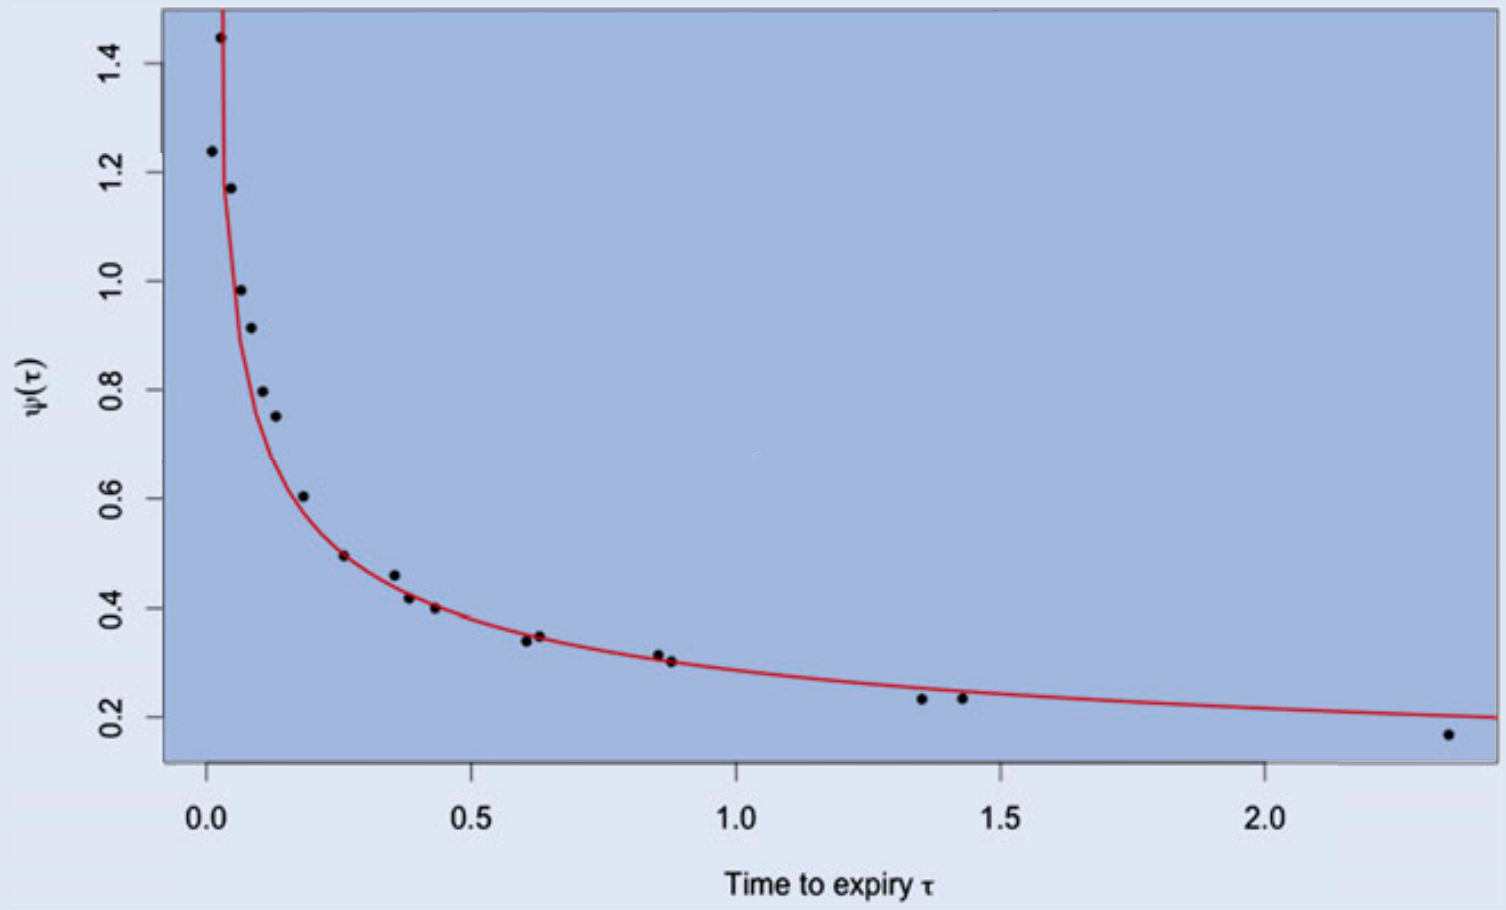
\includegraphics[width=0.85\textwidth ]{figs/Bayer2016_fig2.png}
    \caption{Extracted from Bayer et al., 2016  \cite[Figure~2]{Bayer2016}. Plot shows change in volatility skew $\psi(\tau)$ with respect to $\tau$, time to expiry measured in years. The points represent non-parametric estimates of the S\&P ATM volatility skews as of 14/08/13. Red curve is the power-law fit $\psi(\tau) = A\tau^{-0.407}$.}
    \label{fig:Bayer2016_vol_skew}
\end{figure} 

Bergomi and Guyon (2012) derive a small noise expansion for the smile in a stochastic volatility model making use of a forward variance curve, where forward variance is defined as the expectation under the pricing measure of the future instantaneous variance. In this way, given a stochastic model written in the forward curve form, the term structure of ATM skew can be computed easily. The n-factor Bergomi variance curve model can be written as:

\begin{equation}
\label{eq:Bergomimodel}
    \xi_{t}(u) = \xi_{0}(u) \,\varepsilon\,\left[\sum_{i=1}^{n} \eta_{i} \int_{0}^{t} e^{-K_{i}(u-s) dW_{s}^{i}}\right]
\end{equation}

where $\varepsilon_{.}$ denotes the stochastic exponential and $\xi_{0}(.)$ denotes the initial forward variance curve. In this case, the Bergomi model generates a term structure volatility skew of the form:

$$\sum_{i=1}^{} \frac{\eta_{i}}{K_{i}} \Big(1- \frac{1-e^{-K_{i}} \tau}{{K_{i}} \tau}\Big)$$

Thus, to generate the empirically observed form of $\tau^{-\alpha}$ it is expected to replace the exponential kernels in [\ref{eq:Bergomimodel}] with a power-law kernel. Thus, we end up with the rBergomi model which can be simulated as:

\begin{equation}
    S_{t} = S_{0} \,\varepsilon\, \Big(\int_{0}^{t} \sqrt{\nu_{u}} dZ_{u}\Big)
\end{equation}
\begin{equation}
    \nu_{u} = \xi_{0}(u)\, \varepsilon \, \Big( \eta_{i} \sqrt{2H} \int_{0}^{u} \frac{1}{(u-s)^{\gamma}} dW_{s}\Big)
\end{equation}

The rBergomi model is a non-Markovian generalisation of the Bergomi model. This model consists of only three parameters: $H, \eta$ and $\rho$, where the later represents the correlation between volatility moves and prices moves. The parameters mentioned can be interpreted as:

\begin{itemize}
    \item $H$ which controls the decay of ATM skew for very short maturities.
    \item $\rho \eta$ which defines the level of ATM skew for longer maturities.
    \item keeping $\rho \eta$ but decreasing $\rho$, towards to be negative, makes the minimum of each smile move to higher strikes.
\end{itemize}

In Figure \ref{fig:Gatheral2018Talk_fig8}, it is shown how rBergomi model fits the SPX option market. The data was taken on Wednesday prior to expiration of the given options, in order to make the shortest expiration smile more meaningful. Parameters chosen for this day were: $H = 0.05, \eta = 2.3$ and $\rho = -0.9$. It is impressive how only using three parameters, we could get a good fit of the whole SPX volatility surface. It is worth to mention, that rBergomi model did pretty well for extreme short-dated smile and there was no necessity of adding jumps to the model.

\begin{figure}[htpb]
    \centering
    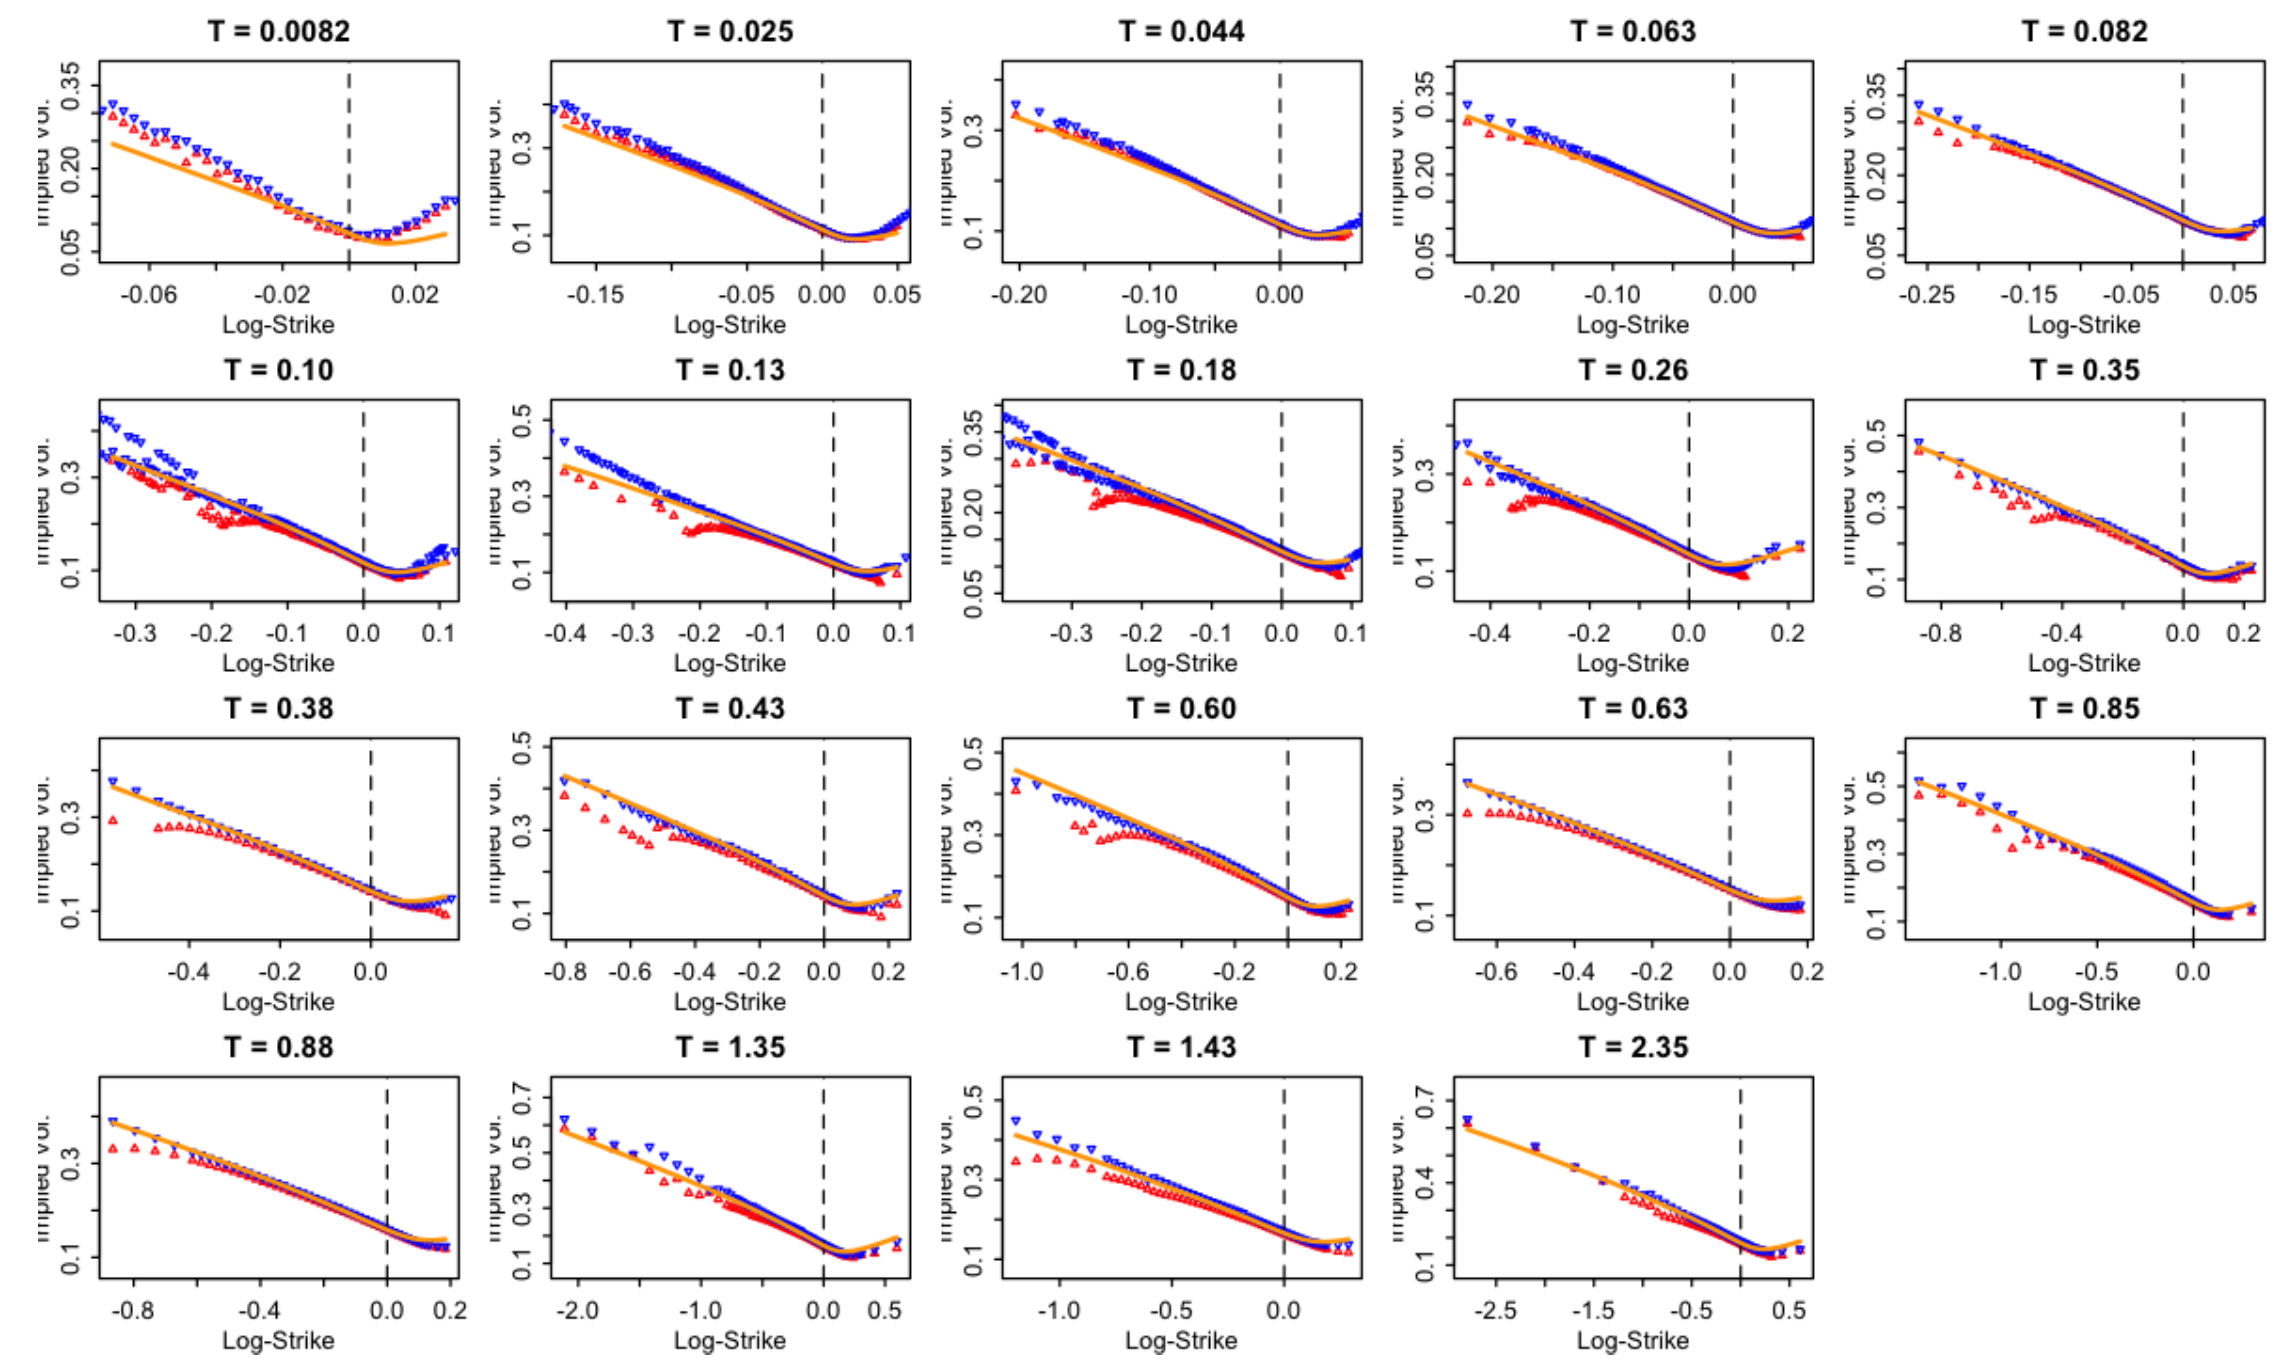
\includegraphics[width=1.0\textwidth ]{figs/Gatheral2018Talk_fig8}
    \caption{Extracted from Gatheral (2018) presentation to Baruch college \cite[Figure~8]{Gatheral2018Talk}. Comparison of implied volatilities of SPX and rBergomi model. Red points represent the bid offer, blue points represent the ask offer and orange lines correspond to the rBergomi simulation.}
    \label{fig:Gatheral2018Talk_fig8}
\end{figure}

\subsection{The Rough Heston Model}
\label{subsec:rough_heston}
The classical Heston model has been introduced, as have the pitfalls  of these simplistic early option pricing models. The classical Heston model does not agree with time series in practice, and does not generate a volatility surface similar to that observed. However, there are flexibility benefits to a model with additional parameters, particularly when applying a rough volatility framework. Small Hurst parameters & fBM are introduced, and the Ricatti characteristic function can be replaced with with a fractional Ricatti characteristic function to form the rough Heston model, producing behaviour seen in both historical & implied volatility. This has been well discussed in \cite{OElEuch2018} and \cite{ElEuchRosenbaum2019}.
\\

Before describing why Rough Heston models produce accurate implied volatility models, we must first introduce Hawkes process. A Hawkes process is a class of stochastic process, pleasantly articulated in \cite{Laub2015}, which has a `self-exciting' characteristic, whereby each time step, or `arrival' over time, within a process leads to excitement which gives a greater probability of exaggerating the characteristics of the process experienced at current time step in the subsequent time step. When a Hawkes process is interpreted as a model of a tradeable asset price over time, it is clear to see how this can be successfully applied to the fickle behaviors of financial markets, i.e. where large volumes of sales/buying of an asset leads to further selling/buying, and the resulting sensational decrease/increase of the asset price. This behaviour is most famously seen in large financial crashes (the 2008 financial crisis, Brexit, flash crash of 2010), or short term economic bubbles, and can be seen in Figure \ref{fig:gatheral_2014_volplots}. 
\\

By sequencing a large number of Hawkes type point processes in \cite{Omar2016}, it was found that these converge to a rough Heston model over the long run, with careful construction considerations. Micro-structures of the rough Heston were created via ultra-high-frequency Hawkes style price model sequences using the following stylised facts of the modern markets: 

\begin{enumerate} 
\item The majority of orders in the market are reactive algorithmic trades with no true economic rationale (described as highly endogenous). 
\item Arbitrage scenarios are highly unlikely due to the high frequency nature of the orders made in the market.  
\item Large algorithmic transactions, split over time and not in one order, make up a large proportion of transactions in the market.
\item There is bid-ask asymmetry: markets shall react differently to a market maker selling an asset as opposed to buying. The price in the market of a given asset shall likely increase when a market maker buys this asset, however the change in the assets market price is likely to be of greater (negatively) upon a market maker selling this asset. This is a result of the availability of this asset in the market reduces upon a buying, but increases when sold.  
\end{enumerate}

Prior to defining the Rough Heston model we must return to the fBM in Section \ref{sec:fractionalBm} and $(\textit{$W^H_t$})$, with Hurst parameters $\textit{H} \in (0,1)$, from Section  \ref{sec:rough_vol_evidence}, to be represented in the Mandelbrot - Van Ness representation:

\begin{equation}
\label{eqn:MvN_Hurst}
{W^H_t} = \frac{1}{\Gamma(H + \frac{1}{2})} \int_{0}^{-\infty} ((t-s)^{H-\frac{1}{2}} - (-s)^{H - \frac{1}{2}})W^H_s + \frac{1}{\Gamma(H + \frac{1}{2})} \int_{0}^{-\infty} (t-s)^{H-\frac{1}{2}}W^H_s
\end{equation}


We can see how influential  the kernel  $(t-s)^{H-\frac{1}{2}}$ is within rough volatility dynamics when $H<\frac{1}{2}$, and that the process,
$$\int_{0}^{-\infty} (t-s)^{H-\frac{1}{2}} dW^s$$
has Holder regularity for $H - \epsilon$, for any $\epsilon>0$. El Euch et al.incorporated this kernel, $(t-s)^{\alpha-1}$, to the classical Heston model to introduce a rough volatility-type model, defining the rough Heston Model.

\begin{equation}
\label{eqn:rough_heston}
v_t = v_0 + \frac{1}{\Gamma(\alpha)} \int_{0}^{t} (t-s)^{\alpha-1} \kappa (\theta - v_s)ds + \frac{1}{\Gamma(\alpha)} \int_{0}^{t} \xi\sqrt{v_s}dW_s^{v}
\end{equation}


Where $\alpha = H+\frac{1}{2}$ and $\kappa, \theta, v_0$ and $\xi$ are all positive, and $\rho$ continues to be the correlation coefficient of the two Brownian motions and are all equivalent to Equation [\ref{eqn:classic_heston_var}]. This model was found to be well defined when ${\alpha} \in (\frac{1}{2},1)$ the volatility trajectories almost surely have Holder regularity $\alpha - \frac{1}{2} -\epsilon$, as for Equation [\ref{eqn:MvN_Hurst}], where for any $\epsilon>0$. It is important to note that when $\alpha$ = 1 we achieve the classical Heston Model.
\\

To continue with a selected Hurst parameter of $H < \frac{1}{2}$ as per Gatheral et al. \cite{Gatheral2014}. The Rough Heston model will be non-Markovian and $v_t$ is no longer a semi-martingale, which as stated \ref{sec:fractionalBm} introduces smoothness to the model. This provides perfect motivation for El Euch et al., to design micro-structures of Hawkes point processes to model the `nearly unstable' behaviour of past events, and go on to demonstrate that combining the convergence results of these processes yield the characteristic function of the log-price of the rough Heston model. The suitability of these results can be seen in Figure \ref{fig:elEuch_1}.
\\

\begin{figure}[htpb]
    \centering
    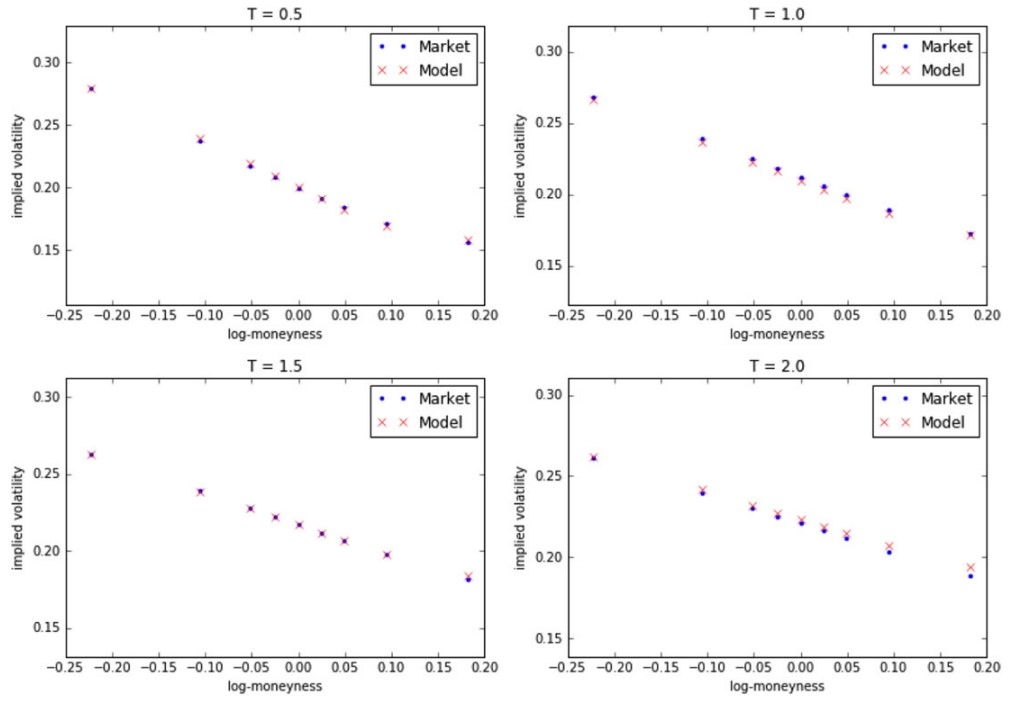
\includegraphics[width=0.9\textwidth ]{figs/Omar2016_fig51.jpg}
    \caption{Extracted directly from El Euch and Rosenbaum, 2016, \cite[Figure~5.1]{Omar2016}. Implied volatility surface generated from a rough Heston model with careful calibration ($\alpha=0.62$)has been shown to have close approximation to historical volatility on S\&P (January 2010) for varying maturity dates (T).}
    \label{fig:elEuch_1}
\end{figure}

One additional note on the suitability of the rough Heston model is that the  "self-exciting" characteristics which the Hawkes micro-processes which jump in probability based on past events negates considerations of introducing any "jump processes" (same as for rBergomi model), which are generally discouraged in modern models. 
\\

The models described in this section are all reliant on significant computational effort in order to do accurate pricing, as they all require calibration in order to find parameters that are representative of the market. In the next section we give a short account of improvements made that help with this.

\section{Computational Cost Reduction}
\label{sec:comp_advancement}
Moving to a more generalised setting, we now focus on rough volatility models as an overall concept that we know are driven by fBM. As mentioned in \cite{Jacquier2020}, the use of fBM in such models carries a computational burden. Pricing via Monte Carlo simulation of the asset price and volatility processes is one pricing tool that functions well, but it can be slow in approximating continuous time solutions within a sufficient level of accuracy. This is particularly true for simulating non-Markovian processes due to the extra memory required to store previous process states. Here, we give a brief overview of some work that introduces potential ways to combat the computational expense of exact Monte Carlo simulation of the volatility process. Namely, we discuss the Hybrid scheme \cite{Bennedsen2017}, the Markovian representation of fBM \cite{Harms2020} and the extension of the Donsker theorem to fBM \cite{Horvath2019}. These methods were introduced to improve the efficiency of the simulation of fBM and rough volatility processes while maintaining good levels of accuracy.

\subsection{The Hybrid Scheme}
\label{subsec:hybrid_scheme}
The Hybrid Scheme was introduced in \cite{Bennedsen2017} in which they study simulation methods for Brownian semistationary processes. A Brownian semistationary process is given by Equation \ref{eqn:semistationary}. 

\begin{equation}
\label{eqn:semistationary}
X(t)=\int_{-\infty}^t g(t-s) \sigma(s) dW(s),  \ \  t\in\mathbb{R},
\end{equation}

where $\sigma_t$ is a predictable process with respect to the given filtration, $W$ is a standard Brownian motion and g is a deterministic function. It is mentioned in \cite{Bennedsen2017} that when $g(x) \propto x^\alpha$ and $\alpha \in (-\frac{1}{2}, \frac{1}{2}) \setminus \{0\}$, the process behaves (locally) like a fBM with Hurst parameter $H=\alpha+1/2$.  Therefore, being able to efficiently simulate such a process would help to improve computational efficiency for simulation in some rough volatility models.  
\\

The Hybrid scheme involves approximating the function $g$ using a step function except for near 0, where a power function is used for approximation. This is a build upon the Riemann sum scheme where no power function is used near 0. Through a series of derivations, the resulting discretisation scheme is written as a linear combination of a Riemann sum and Wiener integrals. The scheme is given by Equations
\ref{eqn:hybrid1}-\ref{eqn:hybrid4}.  
\begin{equation}
\label{eqn:hybrid1}
X_n(t) = \hat{X}_n(t) + \tilde{X}_n(t)
\end{equation}
where,
\begin{equation}
\label{eqn:hybrid2}
\hat{X}_n(t) = \sum_{k=1}^{\kappa} L_g(\frac{k}{n}) \sigma (t-\frac{k}{n}) \int_{t-\frac{k}{n}}^{t-\frac{k}{n}+\frac{1}{n}}(t-s)^\alpha dW(s),
\end{equation}
and,
\begin{equation}
\label{eqn:hybrid3}
\tilde{X}_n(t)=\sum_{k=\kappa+1}^{N_n}g(\frac{b_k}{n})\sigma(t-\frac{k}{n})(W(t-\frac{k}{n}+\frac{1}{n})-W(t-\frac{k}{n})),
\end{equation}
with $L_g$ chosen so that,
\begin{equation}
\label{eqn:hybrid4}
g(t-s) \approx (t-s)^\alpha L_g(\frac{k}{n}), \ \ t-s \in [\frac{k-1}{n},\frac{k}{n}]
\end{equation}

The key takeaway from Equations \ref{eqn:hybrid1}-\ref{eqn:hybrid4} is to highlight that this scheme builds on the Riemann sum scheme by including Equation \ref{eqn:hybrid2}, which approximates $g$ near 0. The inclusion of this term reduces the root mean square error by a significant amount and it is only needed to capture the steepness near 0, so setting $\kappa$ to be small will do this sufficiently while maintaining a low computational cost. In terms of applying the scheme to rough volatility models, the Hybrid Scheme was used for option pricing in the Bergomi model via Monte Carlo simulation, as is discussed in the referenced paper. Using the Hybrid Scheme in this setting simplified the simulation process and reduced the computational cost compared to producing exact simulations from the model \cite[Page~20]{Bennedsen2017}. The results from using the scheme were then compared to exact results from the Bergomi model and it showed that the Hybrid Scheme was able to produce almost exactly the same volatility surface as that produced by exact simulation from the Bergomi model while being significantly more efficient.

\subsection{Markovian Representation of fBM}
\label{subsec:markovian_rep_fBm}
Without going into too much detail, it was shown in \cite{Harms2020} that fBM can be approximated by a Markovian representation consisting of the sum of $n$ weighted Orstein-Uhlenbeck processes. Based on a set of assumptions outlined in the paper, the approximation is given by Equation \ref{eqn:markov_approx}.

\begin{equation}
\label{eqn:markov_approx}
W_t^{H,n} = \sum_{i=1}^n w_{n,i} \int_0^t e^{-(t-s)x_{n,i}}dW_s, \ \ t \in [0,T], 
\end{equation}

where the $x_{n,i}$ are so-called `speeds of mean reversion' and the $w_{n,i}$ are weights, with both terms taking strictly positive values. This approximation forms part of a theorem which states that for any $n\in\mathbb{N}$ and any given $r\in(0, \infty)$, there exists $w_{n,i}$ and $x_{n,i}$, $1\le i\le n$, such that $W^{H,n}$ converges to $W^H$ at a rate of $n^{-r}$. As a consequence, put prices in the Bergomi model also converge at a rate of $n^{-r}$. 
\\

The key takeaway here is that this representation is Markovian since it is a weighted sum of $n$ Orstein-Uhlenbeck process which are both stationary and Markovian. A discrete Monte Carlo scheme for the rough Bergomi model can then be achieved and since the representation is Markovian, it improves efficiency. It is also mentioned that in terms of error and complexity, this method outperforms several other computational methods. However, it is outperformed by the Hybrid Scheme that was discussed earlier. 

\subsection{Extension of Donsker's Theorem to fBm}
Like the previous examples, the motivation of extending Donsker's theorem for Brownian motion to fBm is to be able to approximate fBm in a way that would reduce computational cost. To give some context, we state Donsker's Theorem.
\\

 \noindent\textbf{Theorem (Donsker)}: \emph{Let} $\epsilon_1,...,\epsilon_n$ \emph{be i.i.d. random variables with mean 0 and variance} $\sigma^2$. \emph{Define} $X^{(n)}$ {by}
 \begin{equation}
 \label{eq:donsker_thm}
 X_t^{(n)} = \frac{1}{\sigma \sqrt{n}} (S_{\lfloor nt \rfloor} - (nt - \lfloor nt \rfloor) \epsilon_{\lfloor nt \rfloor + 1}), \ \ t\in[0,1]
 \end{equation}
 \emph{where,}
\begin{equation}
S_m = \sum_{i=1}^m \epsilon_i
\end{equation}

\emph{Then} $X_t^{(n)} \rightarrow W_t$ \emph{in distribution for} $t\ge0$ \emph{on the space of continuous functions, where} $W_t$ \emph{is standard Brownian motion}.
\\

By being able to extend this theorem to fBm, one could approximate the process using i.i.d. sequences of random variables leading to a simplified simulation process. Again, without going into too much detail, an extension of this theorem was given in \cite{Horvath2017}, approximating the logarithm of the stock price under a rough volatility model under the assumption that the i.i.d. random variables have a finite second moment (variance in this case) and a number of other conditions. In terms of pricing, this approximation could then be applied to fractional binomial trees, which opens the door to pricing American-type options under rough volatility models. However, the branches of such trees generally do not recombine which adds to the complexity of this pricing method.   

\subsection{Further Advancements}
\label{subsec:tech_advancement}

In addition to the aforementioned numerical approximations, it is worth mentioning relevant technological improvements to make the calibration of rough volatility models faster, while maintaining the same accuracy for pricing under this type of models.
\\

 Ongoing improvements in technological availability and computational power have made methods, such as that presented by Horvath et al., \cite{Horvath2019}, increasingly accessible. In this work it is shown that neural networks have a significant impact on the computational burden presented by the simulation of rough volatility processes. The authors show that a speed up factor of approximately 12,500 (on average) can be achieved when using neural networks as opposed to standard Monte Carlo methods when calibrating parameters for rough volatility models. It is worth noting that the use of the neural network approach generalises very well to all types of rough volatility models. 
 \\
 
 Due to the model speedup achieved by the use of neural networks, model calibrations can be achieved on the order of seconds, or milliseconds as is shown in Figure \ref{fig:Horvath2019_fig10_11}. This means that model calibration can be done in a real-time, making pricing fast enough regardless of gradient or gradient free methods, with the clear advantage of correctly fitting empirical data. The details of these methods are not explored here, as only the magnitude of calibration time is of interest. We refer the reader to \cite{Horvath2019} for details.
 
 \begin{figure}[htpb]
    \centering
    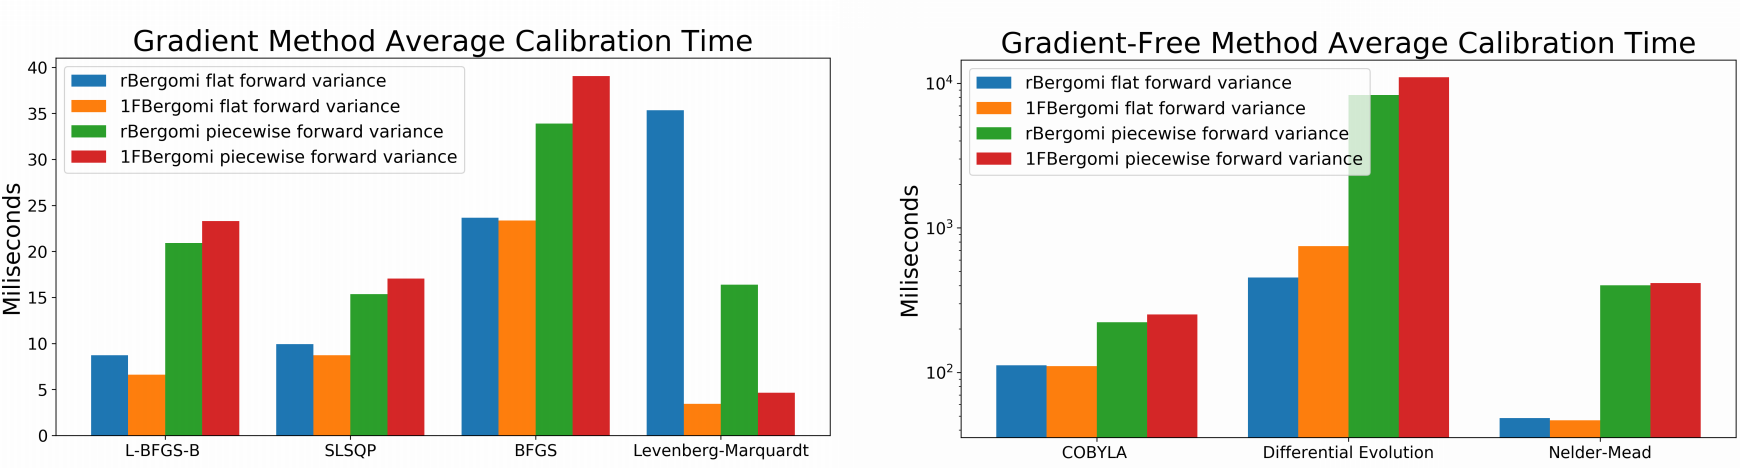
\includegraphics[width=1.0\textwidth ]{figs/Horvath2019_fig10_11}
    \caption{Extracted directly from Horvath et al., 2014, \cite[Figures~10\&11]{Horvath2019}. Plots show that model calibration takes on the order of seconds/milliseconds for both gradient and Gradient-free methods.}
    \label{fig:Horvath2019_fig10_11} 
\end{figure}

\section{Conclusion}
\label{sec:summary&futurework}
 
This report has described the importance of, and the motivation behind, the notion that volatility should not be considered as constant or deterministic as is done in the original Black-Scholes model. We learn in Section \ref{sec:rough_vol_evidence} that volatility can be well represented as a stochastic process, i.e. it possesses its own non-deterministic dynamics. However, standard stochastic models do not exhibit a good fit to the empirical volatility surface. This is a key result that led to rough volatility models being widely accepted.
\\

Gatheral et al. \cite{Gatheral2014} presented evidence from the market data where the increments of the log-volatility process were seen to exhibit a scaling property in expectation with a constant smoothness parameter $H$, almost identical to the scaling property which fBm satisfies. This motivated the modelling of the volatility process using fBm. The innovation that led to the new `rough volatility model' was to consider the Hurst parameter $0<H<1/2$ and that the increments of the fBm are negatively correlated. Using the RFSV model discussed in Section \ref{sec:rough_vol_evidence}, we saw how simulated data produced by such rough volatility models produce a striking resemblance to the observed volatility in a number of ways, see Figure \ref{fig:gatheral_2014_volplots}. In the same way, using this type of model, it was shown a better fit to the ATM skew, especially for short maturities.  
\\

In Section \ref{sec:Pricing}, it was shown how Rough Volatility models can  be  used  to  price  contingent  claims  and  thus  for  pricing options. This was done by performing a change of measure from the physical measure to the risk-neutral measure (using Girsanov's theorem), raising the concept of the price of volatility risk from the change of measure formula. This enables us to make stochastic models rough, such as the rough Heston volatility model or the `rBergomi' model. It is worth mentioning that both model types do not require jump processes yet demonstrate the same unpredictable jumping characteristics when achieving a better fit to the empirical data.
\\

Although rough volatility models have been shown to deliver encouraging results when comparing to market data, the calibration of parameters for such models, as well as simulation using these models are liable to have a relatively high computational cost. Even though Monte Carlo methods are widely used for the simulation of any stochastic process (e.g. for pricing), these methods can be generally quite slow. In Section \ref{sec:comp_advancement}, we present several numerical schemes that reduce the computational cost of Monte Carlo simulation. The Hybrid Scheme is an improvement on the Riemann sum scheme whereby it captures the steepness of the function $g$ near zero in a Brownian semistationary process, while still maintaining a relatively low computational cost. fBM falls into this categories of processes under certain settings, which allows us to apply this scheme directly to fBm. The Markovian representation of fBm allows us to approximate fBm by a weighted sum of $n$ Orstein-Uhlenbeck processes which converges to the true solution, giving the Markovian property that is desired for efficient simulation. And finally, the extension of the Donsker's theorem to fBm enables us to approximate fBm using a sequence of i.i.d. random variables, which also gives us the desired Markovian property. In the same way, improvements in computational power has made the use of neural networks more accessible. As discussed in Section \ref{subsec:tech_advancement}, a speed up factor of approximately 12,500 on average can be achieved compared to using standard Monte Carlo methods.
\\

Advancements, such as those mentioned in Section \ref{sec:comp_advancement}, in overcoming the the computational burden that comes with modelling of rough volatility have created an active area of research. Work in this particular area continues with the aim of being able to use rough volatility models for key financial purposes, such as pricing and risk management, while minimising the computational penalties that arise from such models. 

\bibliographystyle{amsrefs}
% \bibliographystyle{unsrt}
%  \bibliographystyle{plain}  % Or use the `amsrefs' package (http://www.ams.org/tex/amsrefs.html)!
\bibliography{my_bibtex_file.bib}
 \addcontentsline{toc}{section}{Bibliography}
\end{document}
